\documentclass[letterpaper, 12pt]{report} %if any errors, there was a notitlepage after 12pt
\usepackage[colorlinks=true, urlcolor=cyan, citecolor=black, linkcolor=black]{hyperref}
\usepackage{graphicx}
\usepackage{keystroke}
\usepackage{longtable}
\usepackage{booktabs}
\usepackage[utf8]{inputenc}
\usepackage{amsmath, amsfonts, amssymb}
\usepackage{float}
\usepackage{txfonts}
\usepackage{listings}
\usepackage{multirow}
\usepackage[activeacute, spanish, es-tabla]{babel}
\usepackage[spanish]{varioref}
\usepackage{babelbib}           % spanish bibtex.
\usepackage{epsfig}
\usepackage{sty/utfsm_tesis}
\usepackage{apacite}
\usepackage{bm}
\usepackage{tikz}
\usepackage{pgfplots}
\usepackage[flushleft]{threeparttable}
\usepackage{listings}

\pgfplotsset{compat=1.16}
\usetikzlibrary{shapes.geometric, arrows}
\usetikzlibrary{babel}

%Include Table of Contents as the first entry in TOC
\usepackage{sty/xtocinc}

\usepackage[format=plain, labelfont=bf, center]{caption}
\usepackage{subcaption}

\parindent      0.5in
\parskip        2ex

% Fuzz -------------------------------------------------------------------
\hfuzz2pt

\newlength{\defbaselineskip}
\setlength{\defbaselineskip}{\baselineskip}

\newcommand{\setlinespacing}[1]%
	   {\setlength{\baselineskip}{#1 \defbaselineskip}}
\newcommand{\doublespacing}{\setlength{\baselineskip}%
			   {1.3 \defbaselineskip}}
\newcommand{\singlespacing}{\setlength{\baselineskip}{\defbaselineskip}}

\lstloadlanguages{C++, sh, IDL, make}
\lstset{basicstyle=\small\sffamily, commentstyle=\slshape,
        numbers=left, numberstyle=\tiny, numbersep=10pt,
        extendedchars, frame=lines,
        floatplacement=ht, captionpos=b,
        defaultdialect=[CORBA]IDL}

%descomentar para poner fecha distinta a fecha de compilacion
%\copyrightyear{2015} \submitdate{Mes A\~{n}o}
%\convocation{Mes}{A\~{n}o}s

\title{Propuesta metodológica para estimar los beneficios económicos asociados a la coordinación tecnológica BIM en Codelco}
\author{Pascual Soto Uribe}

\begin{document}

%-----------------------------------------------------------------
    %set these plot parameters accordingly
    \pgfplotsset{width=0.8\textwidth, height=0.55\textwidth}

    \renewcommand{\BOthers}[1]{et al.\hbox{}} %para reemplazar y cols. por et al. since I need the English version of babel for it to come by default.
%-----------------------------------------------------------------

    \profguia{Carlos Hunt}
    % \profcorr{Some professor}

    % Archivo de Agradecimientos
    \ack{include/acknowledgements}

    % Incluir Resumen
    \resumenesp{include/resumen}

    % Incluir Abstract
    \resumening{include/abstract}

    % Incluir Abreviaciones
    % \abreviaciones{include/glossary}

    \beforepreface
    \afterpreface

    %\numberwithin{equation}{chapter}

    \chapter{Introducción}
% \addcontentsline{toc}{chapter}{Introducción}

\section{Antecedentes Generales}

\subsection{La Metodología BIM}

BIM es el acrónimo de \emph{Bulding Information Modeling}, que traducido al español quiere decir Modelado de Información de la Construcción, el cual hace referencia al proceso de generación y gestión de datos de una construcción durante su ciclo de vida utilizando algún \emph{software} dinámico de modelado en tres dimensiones y en tiempo real para disminuir la pérdida de tiempo y recursos en el diseño de la construcción. Este proceso produce el modelo de información de la construcción (al que se le conoce como modelo BIM), que abarca tanto la geometría de la construcción, las relaciones espaciales y la información geográfica, así como también las cantidades, las propiedades y atributos de cada uno de los componentes integrados en el modelo.

En otras palabras, el BIM representa un espacio virtual compartido de lo que será construido y su entorno, el que, además, está asociado a las herramientas (\emph{software}), métodos (procedimientos de operación) y análisis (estructural, chequeo de interferencias, construcción, etc.) relacionados con dicho modelo \cite{saldias2010estimacion}.

En esta línea, y para el propósito de esta Memoria, la definición de BIM que mejor se ajusta al trabajo realizado es la que propone el \citeA{nbimstandard}, que postula al BIM como una representación digital de las características físicas y funcionales de un proyecto. Así, el BIM es un fuente compartida de conocimiento e información sobre dicho proyecto, constituyendo una base confiable para la toma de decisiones durante el ciclo de vida de este.

Una premisa básica del BIM es la colaboración entre los actores involucrados durante las diferentes fases del ciclo de vida del proyecto, ya sea para insertar, extraer, actualizar o modificar algún tipo de información en el modelo BIM para apoyar los roles de cada actor.

Así, los requerimientos para que el modelo BIM sea intercambiable están basados en: una representación digital compartida, que la información contenida en el modelo sea interoperable (es decir, que permita intercambios entre distintos computadores), que los intercambios estén basados en estándares abiertos y comunes a la industria, y que los requerimientos de los intercambios puedan ser definidos en lenguaje contractual. %hacer d esto un punteo

En términos prácticos, el BIM puede interpretarse de manera diferente dependiendo de la perspectiva de cada actor:

\begin{itemize}
    \item Aplicado a un proyecto, el BIM representa la gestión de la información. Es decir, los datos contribuidos y compartidos por todos los participantes del proyecto. La información correcta para la persona correcta en el tiempo correcto.
    \item Para los participantes del proyecto, el BIM representa un proceso interoperable para la entrega del proyecto. Es decir, define el trabajo de los equipos y cuántos equipos deben trabajar en conjunto para concevir, diseñar, construir y operar el proyecto.
    \item Para el equipo de diseño, el BIM representa un diseño integrado. Es decir, hace uso de soluciones tecnológicas, incentivando la creatividad, entregando \emph{feedback} y empoderando a los equipos.
\end{itemize}

\subsection{La Construcción en el Sector Minero}

Según lo establecido por la \citeA{inversion-cochilco} en su informe de inversión en la minería chilena, que considera aquellos proyectos con puesta en marcha dentro del período 2018 -- 2027, existen 44 iniciativas avaluadas en unos US\$ 65.747 millones.

Estas 44 iniciativas se pueden dividir en dos grupos: aquellas con una mayor probabilidad de materializarse dentro de los plazos presupuestados, y aquellas cuya probabilidad de materializarse es menor.

Dentro del primer grupo se encuentran las iniciativas en condición base y probable, que suman un total de US\$ 36.257 millones con 25 proyectos, los cuales corresponden a un 55,1\% del total de la cartera.

En el segundo grupo se encuentran aquellos proyectos en condición posible, potencial y los más propensos a verse afectados por cambios en las condiciones de mercado. Corresponden a 19 iniciativas valoradas en US\$ 29.490 millones, que equivalen al 44,9\% del todal de la cartera.

Si se adopta una postura pesimista y sólo se consideran los proyectos del primer grupo, se puede hacer un análisis separado de aquellas iniciativas en condición base y probable. Así, las iniciativas en condición base cuentan con 14 proyectos, cuya inversión asciende a los US\$ 21.931 millones, siendo CODELCO el actor principal con un 68,8\% de la inversión para esta condición. Por otro lado, existen 14 iniciativas en condición probable avaluadas en US\$ 14.326 millones, donde la gran minería privada es la de mayor relevancia con un 91\% del total de la inversión para esta condición.

Para estudiar los montos asociados exclusivamente a la etapa de construcción, se toman en cuenta los porcentajes de impacto en los costos de un contrato EPCM establecidos por CODELCO para cada una de las etapas de dicho contrato. De esta manera, al asociar los porcentajes a los proyectos en condición base y probable se generan los siguientes resultados:

{
\newcolumntype{M}[1]{>{\centering\arraybackslash}m{#1}}

\begin{table}[H]
    \begin{threeparttable} %needed for the table notes
    \centering
    \caption{Impacto en los costos de acuerdo a las etapas de un proyecto EPCM según CODELCO.}
    \label{tab.impacto_ing}
    \begin{tabular}{l M{1.1in} M{1.8in} M{1.5in}}
        \toprule
        \textbf{Etapa} & \textbf{\% de impacto en costos} & \textbf{Proyectos condición base y probable, MM USD} & \textbf{Proyectos condición base, MM USD} \\
        \midrule
        Ingeniería & 10\% & \$ 3.626 & \$ 2.193 \\
        Adquisición & 50\% & \$ 18.129 & \$ 10.966 \\
        Construcción & 35\% & \$ 12.690 & \$ 7.676 \\
        Gestión & 5\% & \$ 1.813 & \$ 1.097 \\
        \bottomrule        
    \end{tabular}
    \begin{tablenotes}
         \small
         \item MM USD = millones de dólares. Fuente CODELCO Chile. 
    \end{tablenotes}
    \end{threeparttable}
\end{table}
}

Tal como se aprecia, la etapa de construcción es la que tiene el segundo mayor impacto en los costos de un contrato EPCM, alcanzando un 35\% de los costos totales de un proyecto.

Así, la inversión asociada a los proyectos en condición base y a la agrupación de proyectos en condición base y probable, representan un $7,35$\% y un $12,16$\% respectivamente del PIB de Chile en 2018\footnote{Dato extraído del Banco Mundial \url{https://datos.bancomundial.org/pais/chile}}.

%Remember to add "extraído por" when citing this shit

\subsection{BIM en Codelco}

%Extraído de https://planbim.cl/codelco-adhiere-a-planbim/?lang=en

Tras un proceso gradual de implementación de metodologías y tecnologías BIM ---que partió en 2010 con la incorporación de procesos de gestión documental y empleo de modelos 3D para el diseño de proyectos estructurales y de mantenimiento de instalaciones, en los que se entendía el BIM no sólo como un software, sino como una forma de gestionar información--- Codelco suscribe el ``Acuerdo de Colaboración y Complementación de Capacidades para Incrementar la Productividad de la Industria de la Construcción'' con Planbim de Corfo en 2018 con el fin de aumentar la productividad y eficiencia en sus proyectos.

El convenio busca fomentar la incorporación de procesos, estándares y tecnologías de información y comunicaciones, junto con metodologías BIM, para generar un cambio metodológico que integre habilidades y capacidades a los trabajadores mediante el uso de nuevas tecnologías y trabajo colaborativo e interdisciplinario, que permitan la integración de la gestión de proyectos y el manejo optimizado de información a lo largo del ciclo de vida completo de los activos, desde su diseño hasta su operación.

%--
Así, y con el fin de convertirse en la institución que realiza los proyectos más productivos del país, es que Codelco emitió un mandato corporativo durante el primer semestre del 2019, en el que se indica el uso obligatorio de la metodología BIM para todos los proyectos de la corporación.

\section{Motivación}

Las iniciativas en estado base y probable proyectadas para el período 2018 -- 2027 representan un $12,16$\% del PIB nacional del año 2018. Asimismo, de acuerdo las ponderaciones mostradas en la Tabla \ref{tab.impacto_ing}, los costos asociados a la etapa de construcción de estos proyectos representa un $4,26$\% del PIB registrado en 2018.

Tales cifras muestran la importancia de diseñar, construir y gestionar los proyectos de manera eficiente. Para ello, Codelco ha establecido el uso del BIM con el fin de, entre otros, ajustarse a los costos inicialmente proyectados como presupuesto base.

Sin embargo, hasta ahora no existe una manera cuantitativa de estimar si el uso del BIM efectivamente contribuye a ajustarse a los costos inicialmente presupuestados, o bien cuál es el beneficio económico asociado al uso de dicha tecnología. Esta falencia es la que ha motivado la realización de este estudio.

\section{Objetivos}

\subsection{Objetivo General}

\begin{itemize}
    \item Proponer un método cuantitativo para estimar el beneficio económico asociado al uso del BIM, proyectando los sobrecostos de un proyecto respecto de su presupuesto inicial según el nivel de madurez BIM alcanzado por dicho proyecto.
\end{itemize}

\subsection{Objetivos Secundarios}

\begin{itemize}
    \item Proponer un indicador de madurez BIM que relacione la desviación en los costos de un proyecto y según su nivel de madurez.
    \item Desarrollar un \emph{script} para mejorar la estimación de los parámetros de la relación entre madurez BIM y desviación en los costos.
\end{itemize}

\section{Alcances del Estudio}

Para el desarrollo de este trabajo se consideró la desviación de los costos asocidada a la etapa de construcción de los proyectos estudiados, la que fue extraída del detalle de los contratos en sus etapas iniciales y finales. Esto de acuerdo al requerimiento establecido por Codelco, cuya prioridad era conocer el impacto de la implementación del BIM en los costos de construcción de un proyecto.

Además, la muestra sobre la que se trabajó es muy acotada ---tres proyectos de construcción de plantas minero-industriales---, sin embargo, el fin de este estudio no es entregar un modelo cuyo rigor estadístico permita su generalización, sino más bien proveer una metodología capaz de predecir los sobrecostos de un proyecto bajo cualquier contexto (construcción industrial, construcción comercial, etc) considerando solamente su nivel de madurez BIM, independiente de la escala que use para medirla.


\section{Metodología de Trabajo}

El desarrollo de la propuesta aquí presente se realizó de la siguiente manera:

\begin{itemize}
    \item Proposición del tema por parte de Codelco. Codelco necesitaba conocer de manera cuantitativa las ventajas de la utilización del BIM, dado que el uso de la tecnología BIM estaba asociada a una ``sensación'' de ahorro que necesitaba ser cuantificada.
    \item Revisión bibliográfica y búsqueda en la literatura para conocer las maneras de medir cuantitativamente los beneficios asociados a la implementación del BIM en los diferentes proyectos de construcción en el mundo.
    \item Reuniones semanales con el jefe del área BIM en Codelco para evaluar los avances en la propuesta y recibir \emph{feedback} sobre el trabajo realizado.
    \item Minería de datos para establecer los sobrecostos en los proyectos estructurales realizados con BIM en la Vicepresidencia de Proyectos y así poder generar un vector de desviaciones en los costos de cada de los proyectos en la etapa de construcción.
    \item Reuniones con el experto y coordinador BIM de los proyectos estudiados para conocer el \emph{rating} de madurez de cada proyecto con el fin de generar un vector de \emph{ratings} de madurez BIM.
    \item Desarrollo de un indicador de madurez consecuente con la relación inversa entre madurez BIM y desviación de en los costos de un proyecto.
    \item Utilización de técnicas predictivas, en particular, mínimos cuadrados ordinarios, para generar un modelo capaz de predecir las desviaciones de costos en la etapa de construcción de los proyectos de acuerdo al nivel de madurez BIM alcanzado por cada uno de ellos.
    \item Presentación de resultados ante comisión experta de la Cámara Chilena de la Construcción, el jefe BIM de codelco y el equipo BIM de la Vicepresidencia de Proyectos.
    \item Entrega de informe con las conclusiones y sugerencias pertinentes.
\end{itemize}

\section{Estructura de la Memoria}

El presente trabajo de Memoria se estructura de la siguiente manera:

%completar esto una vez terminado el primer borrador de la Memoria

  
    \chapter{Definición del Problema}

\section{Contexto}


    
    % \chapter{Estado del Arte}

\section{La metodología BIM}

%Thus, \shortcite{lu2014cost} 
Ejemplos con \textbackslash \texttt{cite}: \shortciteA{lu2014cost}; \cite{lu2014cost}; \citeA{lu2014cost} y \citeNP{lu2014cost}.


%%%%%%%%%%%%%%%%%%%%%%%%%%%%%%%%%%%%%%%%%%%%%%%%%%%%%%%%%%%
\subsection{Ventajas de la metodología BIM}

La metodología BIM, considerada como plataforma de coordinación, puede tener dos efectos en el comportamiento de un contrato \cite{chang2014economic}: 
\begin{enumerate}
    \item Digitalizar el diseño en un conjunto de objetos paramétricos 3D podría reducir la incidencia de malas interpretaciones de la información del diseño provenientes de errores humanos durante la transferencia de información. Digitalizar reduce, de manera inherente, la incidencia en las órdenes de cambio, lo que permite que el dueño del proyecto esté menos expuesto a retrasos en los pagos.
    \item El uso de la metodología BIM podría hacer posible que las empresas subcontratistas incorporasen sus inputs en el diseño digital durante una etapa temprana. Además, el uso de BIM facilita la detección de interferencias que podrían resultar en un cambio durante la etapa de construcción. Todo lo anterior también impacta en la reducción de la exposición a cambios indeseados del dueño.
\end{enumerate}


Mainly a test to see if this shit is working properly

    \chapter{Marco Teórico}

\section{La metodología BIM}

La metodología BIM consiste en un conjunto de tecnologías, metolodogías y estándares que permiten y facilitan el diseño, la construcción y la operación de un proyecto de construcción de forma colaborativa en un espacio virtual compartido \cite{tabilo2019estudio}.

Por otro lado, es común encontrarse con dos definiciones en la literatura que difieren ligeramentea la hora de abordar el BIM en términos conceptulaes. Estas definciones se pueden agrupar y conceptualizar de acuerdo a las siguientes definiciones:

\begin{enumerate}
    \item \textbf{Building Information Model:} representación digital paramétrica del producto de construcción, es decir, losas, muros, pilares, equipamiento, puertas, ventanas, etcétera, que incluye su geometría e información \cite{lnb}.
    \item \textbf{Building Information Modeling:} metodología/proceso  que permite desarrollar y utilizar diversos modelos  de representación digital paramétrica para apoyar decisiones de diseño, construcción y operación durante todo el ciclo de vida de un proyecto, lo que implica una integración y gestión de información provista y usada por diferentes actores del proyecto. De esta manera, se busca disminuir la pérdida tanto de tiempo como de recursos durante el diseño y la ejecución de la obra \cite{bimforum}.
\end{enumerate}

Ambos conceptos son complementarios. En este sentido, no merece la pena hacer distinciones entre uno y otro y se pueden utilizar de manera intercambiable, dado que la metodología BIM requiere de un modelo BIM para su desarrollo. Asimismo, el modelo BIM pierde su potencial si este no se utiliza bajo un marco conceptual adecuado \cite{cardenas2016incorporacion}.

El eje central del BIM es, entonces, la colaboración entre las diferentes partes que conforman las fases del ciclo de vida de un proyecto, y cuya tarea es insertar, extraer, actualizar o modificar información en el modelo BIM para apoyar y reflejar las funciones del proyecto de construcción. Esto permite el flujo de información (cuya particularidad es que se actualiza de manera instantánea), control, supervisión y validación de todos los procesos involucrados. Trabajar de esta manera permite que todos los cambios realizados en el modelo sean de conocidos por todos los \textit{stakeholders} del proyecto \cite{trejo2018estudio}.

Es importante mencionar que, si bien el BIM es una metodología que permite la pronta detección y corrección de errores de cualquier tipo, y que,además, reduce las tareas repetitivas y redundantes, la ingesta de información del modelo es responsabilidad de personas. Son las personas quienes reúnen y e ingresan la información, por lo que no se debe pensar en el BIM como una metodología \textit{error free}.


\subsection{Dimensiones BIM}

Un proyecto concebido bajo la metodología BIM tiene un ciclo de vida que comienza con una idea y termina con la mantención del proyecto. Así, el ciclo de vida de un proyecto BIM se puede dividir en siete fases, que la literatura ha denominado como las dimensiones BIM \cite{tabilo2019estudio}:

\begin{itemize}
    \item \textbf{1D (la idea):} la idea permite definir las condiciones inciales, realizando las primeras estimaciones de sueprficie, volúmenes y costos. También se establece el plan de ejecución.
    \item \textbf{2D (el boceto):} se elije y prepara el \textit{software} para hacer la modelación del proyecto. Se definen los materiales, las cargas estructurales y se establecen las bases para la sostenibilidad del proyecto.
    \item \textbf{3D (modelo de información de la construcción
    ):} con toda la información recopilada se genera el modelo 3D que servirá como base para el resto del ciclo de vida del proyecto. No es sólo un modelo gráfico, sino que además incorpora toda la información que se necesitará para las siguientes fases.
    \item \textbf{4D (tiempo):} se incorpara la variable tiempo. Es decir, se definen las fases del proyecto y la duración de estas. Establece la planificación de los plazos de todo el proyecto.
    \item \textbf{5D (costos):} se incorpora el control de costos y estimación de gastos del proyecto.
    \item \textbf{6D (simulación):} consiste en simular las posibles alternativas del proyecto para finalmente llegar a la alternativa óptima, todo esto antes de comenzar la construcción del proyecto.
    \item \textbf{7D (instructivo):} se establece el manual de la vida útil del proyecto una vez construido, para el uso y mantenimiento de éste.
\end{itemize}


\subsection{Niveles de información BIM}

Existen distintos niveles de información BIM ya sea para el detalle, el desarrollo y la información del proyecto de construcción. Sin embargo, existe un concepto común que agrupa todos los niveles de información existentes. El concepto es el acrónimo LOD. No obstante, el LOD adopta interpretaciones distintas según la fuente de su procedencia. Así, para los estándares de Estados Unidos, definidos por la \textit{National BIM Standard-United Sates\textregistered} (NBIMS-US\texttrademark), LOD hace referencia a \textit{Level of Development}. Por otro lado, los estándares británicos están definidos por la \textit{National Building Specification} (NBS-UK), en los que LOD hace referencia a \textit{Level of Definition} \cite{trejo2018estudio}.

el \citeA{bimforum2} indica que la diferncia fundamental es que el nivel de detalle se incluye en el elemento del modelo (NBS-UK), mientras que el nivel de desarrollo es el grado en que la geometría e información del elemento se ha pensado; es decir, según la fase de diseño del proyecto, por lo que entrega un cierto nivel de confianza para seguir avanzando en el desarrollo del proyecto en el modelo (US).

\subsubsection{Niveles de detalle}

El NBS-UK plantea que el término \textit{Level of Definition} se refiere al nivel de detalle (descripción gráfica de los modelos en cada etapa). Dicha institución también define un \textit{Level of Information} (LOI), que describe el contendo no gráfico del modelo en cada etapa \cite{trejo2018estudio}.

A continuación de describen los LOD e LOI definidos por el NBS-UK de acuerdo a lo señalado por el \cite{bimforum2}:

\begin{itemize}
    \item \textbf{LOD 1:} conceptualización. Casi nula geometría.
    \item \textbf{LOD 2:} el elemento de construcción modelado proporciona una indicación visual del elemento en la etapa conceptual, identificando requerimientos claves como el acceso o zonas libres para el posterior mantenimiento. Esta información es adecuada para la coordinación espacial inicial de los elementos o sistemas.
    \item \textbf{LOD 3:} el elemento de construcción modelado proporciona una representación visual del elemento en la etapa de definiciones técnicas para su coordinación espacial completa.
    \item \textbf{LOD 4:} el elemento de construcción modelado proporciona una representación visual del elemento para una etapa de diseño, con su coordinación espacial completa.
    \item \textbf{LOD 5:} el elemento de construcción modelado proporciona una representación visual del elemento en el proyecto construido y provee una referencia, para su posterior uso y mantenimiento.
\end{itemize}

\begin{figure}[H]
    \centering
    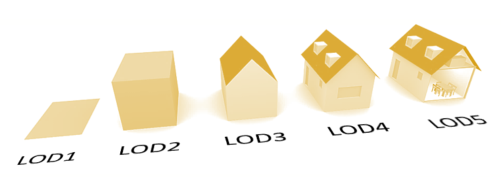
\includegraphics[width=0.65\linewidth]{images/LOD.png}
    \caption{Ejemplo de nivel de definición.}
\end{figure}

\subsubsection{Niveles de información}

Los niveles de información (LOI) definidos por la NBS-UK y descritos por el \citeA{bimforum2} se muestran a continuación:

\begin{itemize}
    \item \textbf{LOI 2 y 3:} el elemento modelado proporciona una descripción inicial para una entrega hacia el diseño.
    \item \textbf{LOI 4:} el elemento modelado proporciona una información suficiente para permitir la selección del producto de fabricante que cumpla con sus requerimientos. Esta información también puede ser utilizada para reemplazar un elemento durante el ciclo de vida del proyecto, una vez construido.
    \item \textbf{LOI 5:} el elemento modelado proporciona la información específica del producto de fabricante seleccionado o lo construido y entregado. Cualquier información adicional pertinente durante el proceso de construcción o instalación es indicada dentro de este nivel.
    \item \textbf{LOI 6:} el elemento modelado proporciona la información acumulada de los niveles anteriores y además considera información detallada del mantenimiento efectuado.
\end{itemize}

\subsubsection{Niveles de desarrollo}

Adicionalmente, el \textit{American Institute of Architects} (AIA) define al nivel de desarrollo como la forma de identificar requisitos mínimos y usos específicos a cada elemento del modelo, en un respectivo nivel. Los siguientes, son los niveles de desarrollo, en base a lo expuesto por el \citeA{bimforum2}:

\begin{itemize}
    \item \textbf{LOD 100:} el elemento puede ser representado gráficamente en el modelo con un símbolo u representación genérica. Estas representaciones muestran la existencia de un componente, pero no su forma, tamaño o ubicación precisa. La información debe ser considerada aproximada.
    \item \textbf{LOD 200:} el elemento se representa gráficamente como un sistema genérico de objeto, tamaño, forma, ubicación y orientación aproximados. La información no gráfica también es aproximada. Estas representaciones son respecto del volumen o espacio reservado.
    \item \textbf{LOD 300:} el elemento representa gráficamente como un objeto o sistema específico en términos de cantidad, tamaño, forma, ubicación y orientación. La información no gráfica se corresponde con la información gráfica. Las cantidades, dimensiones, formas, ubicación y orientación según lo diseñado se pueden obtener directamente a del elemento.
    \item \textbf{LOD 350:} igual al LOD 300, pero las representaciones se vinculan con otros elementos del modelo cercano o adjunto y se incluyen las partes tales como soportes o conexiones.
    \item \textbf{LOD 400:} LOD 350 más la modelación. Estas representaciones se modelan con la precisión y detalle suficiente para su fabricación e instalación.       
    \item \textbf{LOD 500:} el elemento modelado es una representación fiel del elemento de construcción ya ejecutado en obra, con su tamaño, forma, ubicación y orientación real en el proyecto. La información no gráfica está incluida en el objeto, así como sus vínculos con otros elementos. Estas representaciones se realizan una vez construido el proyecto y son las adecuadas para el mantenimiento y el funcionamiento del elemento en el inmueble.
\end{itemize}

\begin{figure}[H]
    \centering
    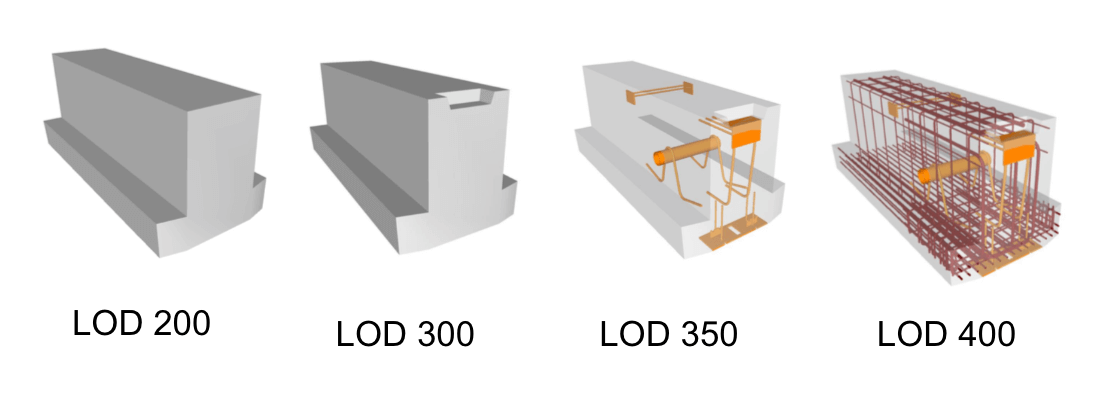
\includegraphics[width=0.95\linewidth]{images/lod-arch.jpg}
    \caption{Ejemplo de nivel de desarrollo.}
\end{figure}

\subsection{Madurez BIM} 

Existen diversos métodos y herramientas para estimar el nivel de madurez BIM de un proyecto. Por ejemplo, la NBIMS-USA\textregistered cuenta con un modelo de capacidades de madurez para definir la madurez de los modelos y permitir a los usuarios evaluar us prácticas y procesos basados en un espectro y funcionalidades técnicas definidas. El objetivo de las capacidades de madurez es proveer criterios de comparación y metas para el progreso en la madurez proyectos. Esta herramienta consiste de diez niveles de madurez, siendo diez el máximo \cite{trejo2018estudio}.

Por otro lado, la NBS-UK propone un modelo que consta de cuatro niveles, los que son \cite{trejo2018estudio}:


\begin{itemize}
    \item \textbf{Nivel 0:} no hay colaboración. CAD 2D solo utilizado en producción. Los \textit{outputs} son distribuidos en papel, en digital o una mezcla de ambos.
    \item \textbf{Nivel 1:} mezcla de CAD 3D para trabajo conceptual y 2D para documentación. Estándares de CAD se administran según BS 1192: 2007 y el intercambio electrónico de datos se lleva a cabo desde un entorno de datos común, a menudo administrado por el contratista. Los modelos no se comparten entre los miembros del equipo del proyecto.
    \item \textbf{Nivel 2:} trabajo colaborativo en que todas las partes usan sus propios modelos CAD en 3D, pero no necesariamente trabajan en un solo modelo compartido. La colaboración tiene que ver con la manera en que se intercambia la información entre las diferentes partes (formato de archivo común).
    \item \textbf{Nivel 3:} colaboración completa entre todas las disciplinas mediante el uso de un único modelo de proyecto compartido que se mantiene en un repositorio centralizado. Todas las partes pueden acceder y modificar ese mismo modelo y el beneficio es que elimina la capa final de riesgo de información conflictiva. Esto se conoce como ``Open BIM".
\end{itemize}

Para \citeA{succar2010building}, la madurez BIM se refiere a la mejora gradual y continua de la calidad, repetibilidad y predictibilidad dentro de una capacidad BIM disponible. La capacidad BIM, por su parte, hace referencia a las habilidades mínimas de una organización o equipo para entregar resultados medibles.

Así, pues, el índice de madurez BIM planteado por Succar consta de cinco niveles de madurez. Estos son: nivel incial, nivel definido, nivel gestionado, nivel integrado y nivel optimizado.

La Vicepresidencia de Proyectos de CODELCO, por su parte, utiliza la definición de Succar para asignar un \textit{rating} de madurez a sus proyectos. Para CODELCO, las cinco etapas definidas por Succar se han modificado someramente para ajustarse sus propias necesidades. Los niveles de madurez para CODELCO son, entonces, los que se detallan a continuación:

\begin{table}[H]
    \centering
    \caption{Niveles de madurez BIM de acuerdo a lo planteado por la Vicepresidencia de Proyectos, CODELCO.}
    \label{tab:niveles-madurez-codelco}
    \begin{tabular}{l p{0.65\linewidth}}
        \toprule
        \textbf{Niveles de madurez BIM} & \textbf{Descripción} \\
        \midrule
        \textbf{Nivel 0} & Nivel inicial pre BIM. Es un diseño a través de planos. \\
        \hline
        \textbf{Nivel 1} & Nivel definido. Consiste en un diseño a través de planos junto a un modelo 3D sin datos adicionales. \\
        \hline
        \textbf{Nivel 2} & Nivel gestionado. Modelo basado en la colaboración. Aquí el diseño es a través de un modelo 3D multidisciplinario con datos y gestión a través de planos. \\
        \hline
        \textbf{Nivel 3} & Nivel integrado. Existe una integración virtual 3D con datos entre distintos contratos de un proyecto, y la gestión a través de de un modelo 3D. \\
        \hline
        \textbf{Nivel 4} & Nivel optmizado. Post BIM. Consiste en un diseño virtual 3D con datos, multidisciplinario, colaborativo y con información integrada entre sistemas. \\
        \bottomrule
    \end{tabular}
\end{table}

Cabe mencionar, sin embargo, que las empresas e instituciones suelen desarrollar sus propios métodos para medir la madurez BIM.

\subsection{BIM en Chile}

El BIM en Chile comenzó su desarrollo desde el ámbito de la arquitectura, expandiéndose a ingeniería, construcción y operaciones. Los primeros indicios del uso de BIM se dieron en la infraestructura hospitalaria, dadas las exigencias en las licitaciones desde el 2009. Dados los beneficios obtenidos en estas experiencias, el BIM se hizo cada vez más atractivos para las demás áreas de la industria \cite{trejo2018estudio}.

El desarrollo de BIM en Chile ha sido monitoreado por distintas entidades, como lo son la CDT, el BIM Forum Chile, universidades, entre otros.

El \citeA{bimforum2}, según sus propias definiciones, es una instancia técnica y permanente, que convoca a los principales profesionales e instituciones relacionadas al BIM en Chile. Busca canalizar las inquietudes técnicas, el conocimiento y la información relacionados a BIM, constituyéndose también en una instancia de desarrollo, difusión y buenas prácticas para el desarrollo tecnológico en el sector construcción.

Los propósitos de BIM Forum Chile son netamente técnicos y sesiona bajo la coordinación de la Corporación de Desarrollo Tecnológico (CDT) de la Cámara Chilena de la Construcción (CChC). También es una instancia abierta y convocante, agrupando a las empresas y profesionales que puedan aportar sus conocimientos y experiencias al mejoramiento de las técnicas relacionadas a BIM.

\subsection{Ventajas de la metodología BIM}

En términos generales, la \citeA{lnb} indica que la principal ventaja es la visualización en 3D de lo que se está proyectando, permitiendo realizar ensayos o probar distintas configuraciones antes de la ejecución, cuantificación automática de cubicaciones, identificación de interferencias, fabricaciones e impulso en la industrialización de la construcción.

En esta línea, la \citeA{lnb} plantea las siguientes ventajas para los usuarios y para el proyecto:

\begin{itemize}
    \item El uso de la metodología y herramientas en general permite establecer un estándar de desarrollo de proyectos, un orden, una mejora de productividad; una vez superada la curva de aprendizaje, mayor rendimiento o menores plazos en el desarrollo de tareas habituales en los proyectos o abarcar más proyectos por la misma cantidad de profesionales, entre otras. El beneficio real que se obtenga de BIM depende de diversos factores, como los objetivos buscados por cada participante, la capacidad de comunicación entre actores, capacidades tecnológicas y humanas de cada oficina, entre otros.
    \item {El uso de BIM en general requiere de un mayor esfuerzo en la fase de diseño de los proyectos, pero esto se retribuye con la posibilidad de realizar ensayos, simulaciones virtuales y distintos tipos de análisis permitiendo la toma de mejores decisiones y más informadas. También se pueden observar menores inconsistencias e interferencias al momento de construir, sin mayores aumentos de plazos y con costos controlados, evitando las ineficiencias por falta de definiciones en el proyecto. Tener múltiples opciones de diseño sin la necesidad de modificar todo el universo de planos o documentación puesto que, al estar vinculadas, la actualización es automática.
    
    Si su uso durante todo el ciclo del proyecto es parte de los objetivos, los beneficios que puede llegar a generar en la planificación de las vías de acceso necesarias para el mantenimiento, en el rastreo y control de los componentes, en remodelaciones y posteriores demoliciones, pueden reflejar un ahorro final significativo en la totalidad de la vida del proyecto desde el punto de vista de la gestión de activos. Cabe destacar que el mayor ahorro de este nuevo proceso se produce en la fase de operación y mantenimiento.} 
\end{itemize}

Por otro lado, el \citeA{bimforum2} indica que:

\begin{quote}
    ``El mayor beneficio se encuentra cuando este modelo y la riqueza de información que incorpora, es usado en conjunto con aplicaciones de administración de edificios o Facilities Management (FM), sobre todo en proyectos complejos que requieren sistemas de apoyo para su funcionamiento como hospitales o industrias, para administrar las mantenciones y costos asociados a estos equipos."    
\end{quote}

Asimismo, la metodología BIM, considerada como plataforma de coordinación, puede tener dos efectos en el comportamiento de un contrato \cite{chang2014economic}: 

\begin{itemize}
    \item Digitalizar el diseño en un conjunto de objetos paramétricos 3D podría reducir la incidencia de malas interpretaciones de la información del diseño provenientes de errores humanos durante la transferencia de información. Digitalizar reduce, de manera inherente, la incidencia en las órdenes de cambio, lo que permite que el dueño del proyecto esté menos expuesto a retrasos en los pagos.
    \item El uso de la metodología BIM podría hacer posible que las empresas subcontratistas incorporasen sus inputs en el diseño digital durante una etapa temprana. Además, el uso de BIM facilita la detección de interferencias que podrían resultar en un cambio durante la etapa de construcción. Todo lo anterior también impacta en la reducción de la exposición a cambios indeseados del dueño.
\end{itemize}


    \chapter{Propuesta}

Si bien el fin de este trabajo es postular un modelo que entregue los lineamientos generales para estimar la desviación en los costos de un proyecto de construcción minero basado en el nivel de madurez BIM 

\section{Métrica propuesta}

Si bien el fin de este trabajo es postular un modelo capaz de estimar los beneficios económicos asociados al uso del BIM en los proyectos de construcción minero-industriales en Codelco, el propósito general es que dicho modelo se pueda extender a cualquier tipo de proyecto de construcción, ya sea minero, industrial, de contrucción habitacional, etc.

%makes a littel sense though, like there's no real connection here

Además, dado el reducido número de proyectos que han adoptado la metología BIM en Codelco, es esencial que el método propuesto desestime el uso de un contrafactual para validarse, puesto que dicho método debe ser capaz de producir un modelo que pueda predecir los beneficios económicos en base al contexto particular de la industria de interés.

En este sentido, un método como el \citeA{barlish2012measure}, donde los indicadores propuestos permiten aventurar conclusiones en base a la comparación del nivel que estos alcanzaron en proyectos con BIM versus proyectos sin BIM, tiene la desventaja de necesitar de un contrafactual para validarse. Por otro lado, un método como el propuesto por \citeA{saldias2010estimacion}, que levanta conclusiones en base a la cantidad de SDIs y órdenes de cambio que pudieron haberse evitado con el uso de la metología BIM, tiene la desventaja de comparar proyectos sin BIM contra el ideal esperado con el uso de BIM, sin tomar en cuenta los puntos intermedios de proyectos que utilizan al menos algún nivel de esta metodología.

Por esta razón, este trabajo propone una metodología y una métrica que toman en cuenta las limitacions mencionadas, es decir, desestima el uso de un contrafactual y considera niveles intermedios del uso del BIM, y que, además, utiliza métodos estadísticos para validarlas.

La métrica propuesta sigue una línea metodológica similar a la mostrada por \shortciteA{lu2012generic}, donde el indicador es un parámetro derivado otros indicadores, que son los esfuerzos (medidos en HH) y la superficie por unidad de trabajo (m$^2$). 

Así, en vez de construir un modelo en base a indicadores que pueden extraerse de manera directa de los reportes de los proyectos, el modelo propuesto utiliza una métrica que toma en cuenta el nivel de madurez BIM alcanzado (de acuerdo a una escala previamente determinada), el nivel óptimo de madurez y la desviación de los costos de los proyectos.

Asimismo, y dado que se espera que los costos de un proyecto crezcan en relación inversa al nivel de madurez BIM alcanzado por este, es necesario que el indicador se compare con respecto a su nivel de madurez óptimo. Formalmente, esto queda:

\begin{equation}
    \text{Indicador Madurez} = \frac{\text{Madurez BIM óptima}}{\text{Nivel madurez BIM}}
\end{equation}

\section{Selección y generación de datos}

\subsection{Criterio de selección}

Para poder generar un modelo que permita validar el uso del indicador propuesto, la información sobre la cuál se compara dicho parámetro es la desviación de los costos en un proyecto determinado, y, en particular, la desviación en costos que tenga relación directa con la falta de integración de la metodología BIM. En otras palabras, la información relevante es la relativa a todos aquellos factores que devinieron en un aumento de costos y que pudieron evitarse de haberse utilizado e integrado el BIM de manera óptima.

De esta manera, la selección de los datos utilizados para relacionar estas variables y generar un modelo capaz de predecir la desviación en costos basasado en la métrica propuesta tuvo dos fuentes principales de las cuales se extrajo la información: el reporte final de los proyectos con los cambios y tendencias, y el detalle de los contratos de cada proyecto.

Sin embargo, dado el nivel de detalle de la información contenida, se escogió el reporte con el detalle de los contratos como fuente de extracción de datos. Además, dicho reporte separa el detalle del costo base y el costo final. Esta clasficiación permite generar una estructuta de filtrado de datos que sigue la siguiente selección jerarquizada:

\begin{enumerate}
    \item \textbf{Contratos que crecieron:} primero, se seleccionan todos los contratos que experimentan un crecimiento en sus costos respecto del presupueto base.
    
    \item \textbf{Sólo crecimientos:} luego, se considera sólo la información referida a los crecimientos de los costos de cada contrato, desestimándose la información detallada sobre el costo base de estos.
    
    \item \textbf{Itemización BIM:} finalmente, se separa la información por ítems relacionados al uso (o falta de uso) de BIM. La itemización BIM se compone de los siguientes ítems: extensión de plazo, obras adicionales, materiales e ingeniería.
\end{enumerate}

La selección de información asociada a cada uno de los ítems de la itemización BIM puede variar según el proyecto. Sin embargo, para el caso de los proyectos analizados en este estudio, las palabras clave para dicha selección eran coincidentes entre proyectos. Esto dado que quienes crean el reporte son parte de la misma Dirección (Dirección de Contratos) y de la misma compañía (Codelco). 

Se tiene, entonces, que para el filtrado por ítem, las palabras clave fueron:

\begin{table}[H]
    \centering
    \caption{Palabras clave para la selección de cada ítem asociado al BIM.}
    \label{tab.keyw}
    \begin{tabular}{ll}
        \toprule
        \textbf{Ítems} & \textbf{Palabras clave} \\
        \midrule
        Extensión de plazo & Extensión plazo, plazo\\
        Obras adicionales & Montaje, obras adicionales, rellenos, reemplazos, reparaciones, etc.\\
        Materiales & Hormigón, piping, cañerías, cables, válvulas, etc. \\
        Ingeniería & Ingeniería, ingeniería de terreno, etc. \\
        \bottomrule
    \end{tabular}
\end{table}

Una vez seleccionada toda la información asociada a cada ítem, se calcula el porcentaje que representa cada uno de ellos respecto del presupuesto base y se genera un nuevo set de datos que representa la desviación en costos asociada al uso del BIM por cada uno de los proyectos.

Luego, las desviaciones en costos para los proyectos estudiados en este trabajo se distribuyen de acuerdo a lo mostrado en la siguiente Tabla:

\begin{table}[H]
    \centering
    \label{tab.datos_desv_proy}
    \caption{Desviaciones en costo de los proyectos estudiados.}
    \begin{tabular}{lccc}
        \toprule 
        Ítem & MH & Molyb & Planta de Ácido \\
        \midrule
        Extensión plazo & 2,0 \% & 5,4 \% & - \\
        Obras adicionales & 19,7 \% & 2,4 \% & 5,6 \%\\
        Materiales & 3,2 \% & 8,1 \% & 5,9\% \\       
        Ingeniería & 0,08 \% & 0,12 \% & 0,3 \% \\
        \textbf{Total} & 25,0 \% & 16,2 \% & 11,8 \% \\
        \bottomrule
    \end{tabular}
\end{table}

\subsection{Herramienta de selección y generación de base de datos}

El reporte con el detalle de los contratos es una planilla Excel con miles de datos, por lo que el filtrado a través de este mismo software no es conveniente. Por esta razón, se creó un código en Python para la selección de los datos requeridos a través de una pseudo minería de datos \footnote{Disponible en \url{www.github.com/psotou/contract-data-selection.git} }. Cabe mencionar que si bien el código se creó para trabajar con cualquier reporte de detalle de contratos emitidos por la Vicepresidencia de Proyectos de Codelco, basta con ajustar algunos parámetros para que dicho código pueda usarse con un reporte de similares características de cualquier otra compañía.

Así, una vez generado el conjunto de datos asociado a las desviaciones en costos, se procede a estimar los resultados arrojados por la métrica propuesta. Para ello, se consultó la opinión experta de Marcelo Vásquez, quien fue el coordinador BIM de todos los proyectos estudiados. 

Ha de mencionarse que la madurez BIM se puede medir usando la métrica o metodología que más convenga, sin embargo, en este estudio se decidió por el uso de la matriz de madurez propuesta por Succar \cite{succar2010building}. Dicha matriz entrega un rating que va del 1 al 4, siendo 4 el óptimo de madurez. Bajo este contexto, la evaluación de Marcelo Vásquez para los proyectos fue la siguiente:

\begin{table}[H]
    \centering
    \label{tab.datos_mad_bim}
    \caption{Nivel de madurez BIM de cada proyecto.}
    \begin{tabular}{lc}
        \toprule 
        \textbf{Proyecto} & \textbf{Nivel de madurez BIM} \\
        \midrule
        Ministro Hales & 1,7 \\
        Moly corporativo & 2,2 \\
        Planta de ácido &  1,8 \\
        \bottomrule
    \end{tabular}
\end{table}

Aplicando la transformación propuesta como indicador (a la que en adelante se referirá como madurez por simplicidad), el conjunto de datos sobre los que se levanta la propuesta de este estudio queda como sigue:

\begin{table}[H]
    \centering
    \label{tab.datos_mad_bim_desv}
    \caption{Base de datos desviación de costos (crecimientos) e indicador madurez.}
    \begin{tabular}{lcc}
        \toprule 
        \textbf{Proyecto} & \textbf{Desviación} & \textbf{Madurez} \\
        \midrule
        Ministro Hales & 25,0 \% & 2,35 \\
        Moly corporativo & 16,2 \% & 1,82 \\
        Planta de ácido & 11,8 \% & 2,22 \\
        \bottomrule
    \end{tabular}
\end{table}


En base a esta información se construye el modelo que permite predecir la desviación en costos de un proyecto de acuerdo a su nivel de madurez BIM.

%-----------------------------MODELO TEÓRICO----------------------
\section{Teoría del modelo propuesto}

En términos generales, la relación entre desviación en costos de un proyecto $i$ y los factores que la motivan se puede expresar de la siguiente manera:

\begin{equation}
    \label{eq.desv-gen}
    y_i = \theta_0 +\sum\limits_{i=1}^n \theta_i x_i
\end{equation}

O bien, de manera vectorial:

\begin{equation}
    \label{eq.desv-vec}
    y_i = \bm{x}^T_i\bm{\theta}
\end{equation}

Donde tanto $y_i$ como $\bm{x}_i$ son variables observadas. Se asumirá que $\varepsilon_i$ (término de error o de perturbación no observado) es absorbido por la constante $\theta_0$. Aquí, $\bm{x}^T$ es un vector fila cuyos elementos son los indicadores de madurez propuestos $(1,~x_1,~x_2,\ldots,~x_n)$, y $\bm{\theta}$ es un vector columna con $(\theta_0,~\theta_1,~\theta_2,\ldots,~\theta_n)^T$  paramámetros desconocidos que son los que se desea estimar para generar un modelo capaz de explicar la influencia de factores tales como el uso de alguna nueva metodología (que es el caso de este estudio), clima, paralizaciones, etc, en la desviación de los costos de un proyecto y, adicionalmente, predecir este resultado.

En este trabajo, $y_i$ representa las desviaciones en costos para el proyecto $i$, y $\bm{x}_i$ es el indicador de madurez propuesto.


Además, la ecuación \eqref{eq.desv-vec} se puede escribir usando notación matricial:

\begin{equation}
    \label{eq.matrix}
    \bm{y} = X\bm{\theta} + \varepsilon
\end{equation}

Donde $\bm{y}$ y $\varepsilon$ son vectores de dimensiones $(N\times1)$, $X$ es una matriz de dimensión $(N\times K)$ y $\bm{\theta}$ un vector de dimensión $(K\times1)$.

Antes de comenzar con la estimación de los parámetros de interés $\bm{\theta}$, se deben levantar algunos supuestos para darle significado al modelo de manera que este no carezca de sentido estadístico. En primer lugar, se asume que las variables explicativas $\bm{x}_i$ son exógenas, lo que implica que $\bm{E}[y_i|\bm{x}_i]=0$. Bajo este supuesto, se sostiene que :

\begin{equation}
    \label{eq.e-xb}
    \bm{E}[y_i|\bm{x}_i] = \bm{x}_i^T\bm{\theta}
\end{equation}

De manera que la curva $\bm{x}_i^T\bm{\theta}$ describe la esperanza condicional de $y_i$ dados los valores de $\bm{x}_i$, y los coeficientes de $\bm{\theta}$ miden cuánto cambia el valor esperado de $y_i$ si cambia un valor $x_{ik}$ (siendo éste el $k$-ésimo elemento del vector $\bm{x}_i$) manteniendo todos los otros elementos de $\bm{x}_i$ constantes (condición ceteris paribus) \cite{verbeek}.

Los parámetros de $\bm{\theta}$ se estimarán on el estimador de Mínimos Cuadrados Ordinarios (MCO). Utilizando la notación de la ecuación \eqref{eq.matrix}, el estimador está dado por:

\begin{equation}
    \label{eq.mco}
    \bm{\hat\theta} = \left( X^TX\right)^{-1}X^T\bm{y}
\end{equation}

Luego, la predicción de valores de desviación vendrá dada por:

\begin{equation}
    \label{eq.predicc}
    \hat{\bm{y}} = X\hat{\bm{\theta}}
\end{equation}

Donde $\hat{\bm{y}}$ son las predicciones de las desviaciones dada la estimación de los parámetros de $\bm{\theta}$.  

La muestra sobre la cual se funda este estudio consiste de un conjunto muy reducido de datos, por lo que se utilizará MCO para muestra pequeña. Las propiedades del estimador MCO para muestra pequeña son:

\begin{align}
    & \label{eq.s1} \bm{E}[\varepsilon_i] = 0\\
    & \label{eq.s2} \varepsilon_i\quad\text{independiente de}\quad \bm{x}_i\\
    & \label{eq.s3} \bm{V}[\varepsilon_i]=\sigma^2 \\
    & \label{eq.s4} \text{cov}[\varepsilon_i,~\varepsilon_j] = 0,\quad i\neq j
\end{align}

El supuesto \eqref{eq.s1} indica que el valor esperado del término de error es cero, esto significa que, en promedio, la curva de regresión debería estar correcta. El supuesto \eqref{eq.s3} indica que todos los términos de error poseen la misma varianza, esto se conoce como homoceasticidad, mientras que supuesto \eqref{eq.s4} impone cero correlación entre los términos de error, excluyende así cualquier forma de autocorrelación. Usando la notación matricial, estos tres supuesto se pueden reescribir de la siguiente forma:

\begin{equation}
    \bm{E}[\varepsilon]=0\quad\text{y}\quad\bm{V}[\varepsilon]=\sigma^2I_N
\end{equation}

Con $I_N$ matriz identidad de dimensiones $(N\times N)$. Esto muestra que la matriz de covarianza del vector de los términos de error $\varepsilon$ es una matriz diagonal con $\sigma^2$ en la diagonal.

El supuesto \eqref{eq.s2} indica que $X$ e $\varepsilon$ son independientes. Este es un supuesto fuerte que implica:

\begin{equation}
    \bm{E}[\varepsilon|X]=\bm{E}[\varepsilon]=0
\end{equation}
\begin{equation}
    \bm{V}[\varepsilon|X]=\bm{V}[\varepsilon]=\sigma^2I_N
\end{equation}

Es decir, la matriz de regresores $X$ no provee ninguna información sobre los valores esperados de los términos de error o sus (co)varianzas. 

Una propiedad muy relevante del estimador de mínimos cuadrados es que se trata de un \textbf{estimador insesgado}. Esto quiere decir que, en promedio, se espera que los valores del estimador $\bm{\hat\theta}$ sean iguales a los valores verdaderos de $\bm{\theta}$ \cite{verbeek}. Formalmente, esto es:

\begin{equation}
    \bm{E}[\hat{\bm{\theta}}] = \bm{\theta}
\end{equation}

Hasta ahora se ha descrito la interpretación del modelo para un valor esperado de $y_i$ dados los valores observado de las variables explicativas $\bm{x}_i$.

Además de ese análisis, es importante conocer el \textbf{efecto marginal} de dichas variables sobre el valor esperado de $y_i$. En otras palabras, en cuántas unidades se espera que cambie $y_i$ si $x_{ik}$ cambia en una unidad siempre que el resto de las variables en $\bm{x}_i$ se mantenga constante (condición ceteris paribus) \cite{hansen2018}. Esta medida viene dada por:

\begin{equation}
    \label{eq.efec_marginal}
    \frac{\partial \bm{E}[y_i|\bm{x}_i]}{\partial x_{ik}} =\theta_k
\end{equation}

%--------------------------MODELO EMPÍRICO---------------
\section{Modelo propuesto}

La coordinación digital de un proyecto de construcción a través del uso de la metodología BIM supone reducir los costos asociados a errores, interferencias, omisiones, etc, por lo que a medida que el grado de integración de la metodología en el proyecto crece, los costos asociados a los problemas mencionados disminuyen.

Dado este escenario, es de esperarse que el uso del BIM impacte de manera postiva en el ahorro en costos de construcción de un proyecto. Se desprende, entonces, que un proyecto que alcanza un buen nivel de madurez BIM debería tener un sobre costo menor al esperado en un proyecto realizado sin BIM.

Por lo anterior, la hipótesis sobre la que se basa esta propuesta es que la desviación de los costos de un proyecto es inversamente proporcional a su grado de madurez BIM. Para ello, se define la variable explicativa $x_{ik}$ de la siguiente manera:

\begin{equation}
    x_{ik} = \frac{m}{m_i}
\end{equation}

Donde $m$ es el óptimo de madurez BIM, y $m_i$ es el nivel de madurez BIM alcanzado por el proyecto $i$. 

Con esto, la ecuación \eqref{eq.desv-gen} queda:

\begin{equation}
    y_i = \theta_0 + \sum\limits_{i=1}^n \theta_i \left(\frac{m}{m_i} \right)
\end{equation}

Además, la desviación en los costos de un proyecto está sujeta las siguientes condiciones de borde de acuerdo a la NBS \cite{nbs}:

\begin{equation}
    y_i = 
    \begin{cases}
        0,33 & \text{si}~~ m_i = m_{\text{máx}} \\
        0,001 & \text{si}~~ m_i = m_{\text{mín}}
    \end{cases}
\end{equation}

La muestra de la que se disponía y sobre la que se trabajó, consistía de tres proyectos minero-industriales, dos de estos proyectos de construcción greenfield mientras que el otro, un proyecto de overhauling. Por esta razón, se realiza un análisis para la submuestra de elementos homogéneos y otro para el total de la muestra.

%--------------------SUBMUESTRA HOMOGÉNEA-------------------------------
\subsection{Submuestra homogénea}

Este análisis considera la submuestra de los proyectos greenfield, que además compartían la construcción del mismo número de plantas de procesamiente, aunque para minerales distintos. Los datos de desviación de costos, madurez BIM y condiciones de borde son los siguientes:

\begin{minipage}{.45\linewidth}
    \begin{equation*}
    Y = 
        \begin{bmatrix}
            0,330 \\
            0,249 \\
            0,161 \\
            0,001 
        \end{bmatrix}
    \end{equation*}
\end{minipage}
\begin{minipage}{.45\linewidth}
    \begin{equation*}
    X = 
        \begin{bmatrix}
            1 & & 4,000 \\
            1 & & 2,353 \\
            1 & & 1,818 \\
            1 & & 1,000
        \end{bmatrix}
    \end{equation*}
\end{minipage}

Esto genera el estimador:

\begin{equation}
    \hat{\bm{\theta}} = 
        \begin{bmatrix}
            -0,0532 \\
            ~~~0,1040
        \end{bmatrix}
\end{equation}

Este resultado genera la siguiente relación:

\begin{equation}
    \label{eq.modelo-prop-submuestra}
    y_i = -0,0532 + 0,104\cdot \left( \frac{4}{m_i} \right)
\end{equation}

Cuyo efecto marginal sobre la desviación esperada de los costos es $0,104$. Es decir, por cada una unidad de madurez BIM se espera una reducción en la desviación esperada de aproximadamente un $10,4\%$.

La escala con la que se mide madurez BIM para este estudio toma valores que van desde el 1 al 4, con un error asociado de $\pm 0,05$. Tomando en cuenta este rating, se genera un gráfico con la predicción de la desviaciones en costos en base al nivel de madurez.

\begin{figure}[H]
    \centering
    \begin{tikzpicture}
        \begin{axis}[
            axis lines = left,
            title = {\textbf{Relación desviación de costos y madurez BIM}},
            ymin = 0, ymax = 0.4,
            xmin = 1, xmax = 4.5,
            xtick = {1, 2, 3, 4},
            ymajorgrids = true,
            grid style = dashed,
            ylabel = Desviación en costos,
            xlabel = Nivel de madurez BIM,
            legend style = {font=\scriptsize},
         ]
        \addplot [
            samples = 100,
            color = purple,
         ]
         {-0.0532+0.104*4/x};
         \addlegendentry{$y_i = -0.0532 + 0.104 \cdot \left( 4\cdot m_i^{-1} \right)$}
        \end{axis}
    \end{tikzpicture}
    \caption{Predicción de la desviación en costos en base a la submuestra homogénea.}
\end{figure}

Las estadísticas asociadas al coeficiente que acompaña la relación de madurez BIM se muestran en la siguiente Tabla:

\begin{table}[H]
    \centering
    \label{tab.est}
    \caption{Estadísticas asociadas al coeficiente de madurez BIM $\theta_1$.}
    \begin{tabular}{lccc}
        \toprule
        Coeficiente & error estándar & $p$-value & $R^2$\\
        \midrule
        0,104 & 0,028 & 0,065 & 0,87\\  
        \bottomrule        
    \end{tabular}
\end{table}

%---------------------MUESTRA TOTAL--------------------------
\subsection{Muestra Total}

Ahora, ingresando los datos de desviación y madurez de toda la muestra, se generan las siguientes matrices:

\begin{minipage}{.45\linewidth}
    \begin{equation*}
    Y = 
        \begin{bmatrix}
            0,330 \\
            0,249 \\
            0,161 \\
            0,118 \\
            0,001 
        \end{bmatrix}
    \end{equation*}
\end{minipage}
\begin{minipage}{.45\linewidth}
    \begin{equation*}
    X = 
        \begin{bmatrix}
            1 & & 4,000 \\
            1 & & 2,353 \\
            1 & & 1,818 \\
            1 & & 2,222 \\
            1 & & 1,000
        \end{bmatrix}
    \end{equation*}
\end{minipage}

Lo que produce el siguiente estimador:

\begin{equation}
    \hat{\bm{\theta}} = 
        \begin{bmatrix}
            -0,0667 \\
            ~~~0,1047
        \end{bmatrix}
\end{equation}

Con lo que la relación entre desviación y madurez se modela como sigue:

\begin{equation}
    \label{eq.modelo-prop-todos}
    y_i = -0,0667 + 0,1047\cdot \left( \frac{4}{m_i} \right)
\end{equation}

Cuyo efecto marginal sobre la desviación esperada de los costos es $0,1047$. Es decir, por cada una unidad de madurez BIM se espera una reducción en la desviación esperada de aproximadamente un $10,5\%$.

El gráfico asociado a la ecuación \eqref{eq.modelo-prop-todos} es:

\begin{figure}[H]
    \centering
    \begin{tikzpicture}
        \begin{axis}[
            axis lines = left,
            title = {\textbf{Relación desviación de costos y madurez BIM}},
            ymin = 0, ymax = 0.4,
            xmin = 1, xmax = 4.5,
            xtick = {1, 2, 3, 4},
            ymajorgrids = true,
            grid style = dashed,
            ylabel = Desviación en costos,
            xlabel = Nivel de madurez BIM,
            legend style = {font=\scriptsize},
         ]
        \addplot [
            samples = 100,
            color = purple,
         ]
         {-0.0667+0.1047*4/x};
         \addlegendentry{$y_i = -0.0667 + 0.1047\cdot \left( 4 \cdot m_i^{-1} \right)$}
        \end{axis}
    \end{tikzpicture}
    \caption{Predicción de la desviación en costos en base a la muestra total.}
\end{figure}

Y las estadísticas asociadas al coeficiente que acompaña la relación de madurez BIM se muestran en la siguiente Tabla:

\begin{table}[H]
    \centering
    \label{tab.est}
    \caption{Estadísticas asociadas al coeficiente de madurez BIM $\theta_1$.}
    \begin{tabular}{lccc}
        \toprule
        Coeficiente & error estándar & $p$-value & $R^2$\\
        \midrule
        0,1047 & 0,027 & 0,03 & 0,83\\  
        \bottomrule        
    \end{tabular}
\end{table}

Si se comparan las curvas generadas a partir tanto de la submuestra como de la muestra total, se puede apreciar un desplazamiento en favor de la curva generada por el modelo derivado de la muestra total (pues se acerca más a las condiciones de borde que indica la teoría).

\begin{figure}[H]
    \centering
    \begin{tikzpicture}
        \begin{axis}[
            axis lines = left,
            title = {\textbf{Relación desviación de costos y madurez BIM}},
            ymin = 0, ymax = 0.4,
            xmin = 1, xmax = 4.5,
            xtick = {1, 2, 3, 4},
            ymajorgrids = true,
            grid style = dashed,
            ylabel = Desviación en costos,
            xlabel = Nivel de madurez BIM,
            legend style = {font=\scriptsize},
        ]
        \addplot [
            samples = 100,
            color = red,
        ]
        {-0.0532+0.104*4/x};
        \addlegendentry{$y_i = -0.0532 + 0.104 \cdot \left( 4\cdot m_i^{-1} \right)$}
        %second plot
        \addplot [
            samples = 100,
            color = blue,
        ]
        {-0.0667+0.1047*4/x};
        \addlegendentry{$y_i = -0.0667 + 0.1047\cdot \left( 4 \cdot m_i^{-1} \right)$}
        \end{axis}
    \end{tikzpicture}
    \caption{Diferencia de predicciones entre el modelo propuesto en base a la submuestra homogénea (línea roja) y a la muestra total (línea azul).}
\end{figure}


%------------RESULTS ANALYSIS----------------
\subsection{Análisis de Resultados}

Como se mencionó más arriba, la propuesta de este estudio se basa en mostrar la relación inversa entre desviación de costos y madurez BIM y, junto a esto, validar la métrica propuesta a través de métodos estadísticos. Así, la hipótesis que se sostiene es que, efectivamente, existe una relación entre estas variables y dicha relación es inversamente proporcional. Formalmente:

\begin{table}[H]
    \begin{tabular}{l p{0.9\linewidth}}
        $H_0$: & La madurez BIM no tiene un efecto inversamente proporcional a la desviación en los costos de construcción de un proyecto. \\

        $H_1$: & La madurez BIM sí tiene un efecto inversamente proporcional a la desviación en los costos de construcción de un proyecto.
    \end{tabular}
\end{table}

Donde $H_0$ es la hipótesis nula y $H_1$ la hipótesis alternativa. 

Para validar el modelo propuesto en términos estadísticos se debe contar con evidencia para rechazar $H_0$. La manera de corroborar dicha información es tomando el cuenta el valor que muestra el $p$-value. Puesto de otra manera, si $p<0,05$ existe evidencia para rechazar $H_0$; de lo contrario, si $p>0,05$, la evidencia en contra de $H_0$ es débil y no se puede rechazar. 

En este caso, y a pesar de lo limitada de la muestra, se tiene que para la submuestra de elementos homogéneos $p>0,05$, por lo que evidencia para rechazar $H_0$ es débil.

Por otro lado, al considerar la muestra total se tiene que $p<0,05$, de manera que se puede rechazar $H_0$ en favor de $H_1$, indicando así que existe evidencia estadística para validar la hipótesis de la relación inversa entre madurez BIM y desviación de costos.

Así, tomando en cuenta el resultado arrojado por la muestra total, el modelo representado en la ecuación \eqref{eq.modelo-prop-todos} sería el adecuado para predecir las desviación en costos de cualquier proyecto considerando únicamente su nivel de madurez BIM respecto de un óptimo. 

Sin embargo, y a pesar de que si bien el resultado de la muestra total se condice con lo esperado en teoría, ha de tenerse en cuenta que se utilizó una muestra bastante acotada, por lo que se debe tener el cuidado pertinente si se quiere generalizar sobre este resultado. No obstante, el modelo propuesto se comporta de manera bastante apropiada y viene a validar, en términos cuantitavos, aquella \emph{sensación} de ahorro que genera la utilización de la metodología BIM.
   
    \chapter*{Conclusiones}
\addcontentsline{toc}{chapter}{Conclusiones}




    %\backmatter
    %\cleardoublepage

    \singlespacing
    \cleardoublepage

    \bibliographystyle{apacite}
    \bibliography{bib/papers}

    \chapter*{Anexos}
\addcontentsline{toc}{chapter}{Anexos}

\section{Matriz de evaluacion de madurez BIM}

\begin{figure}[H]
    \centering
    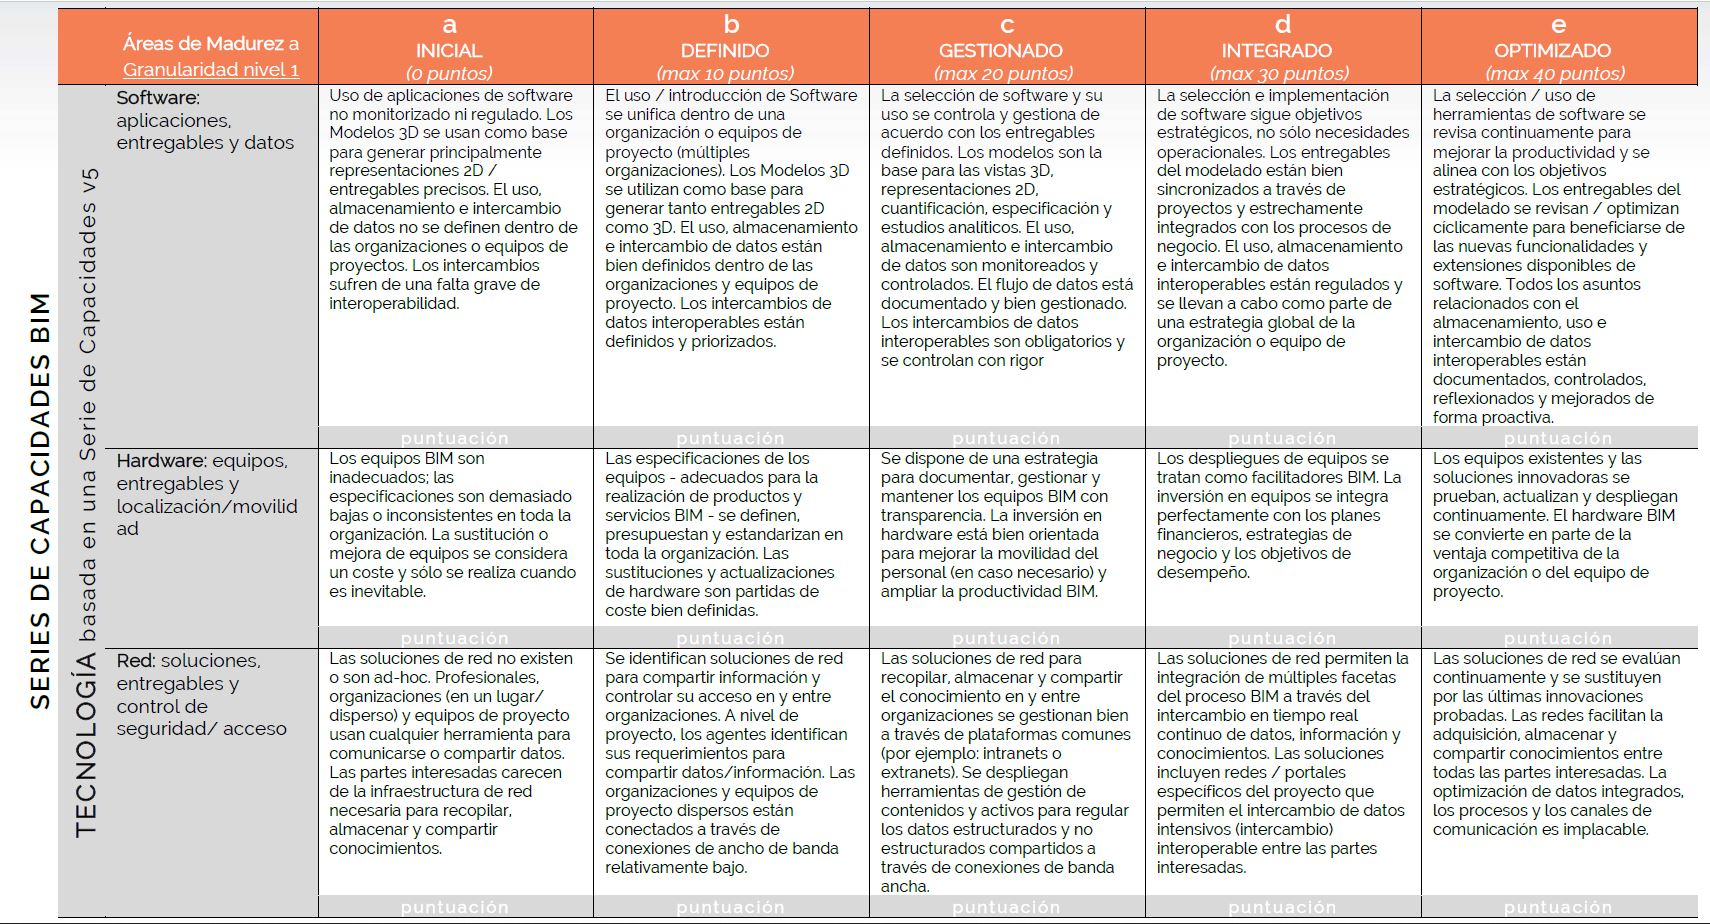
\includegraphics[width=1\linewidth]{images/matriz-madurez-1.jpeg}
    \caption{Matriz basada en la teconología.}
\end{figure}

\begin{figure}[H]
    \centering
    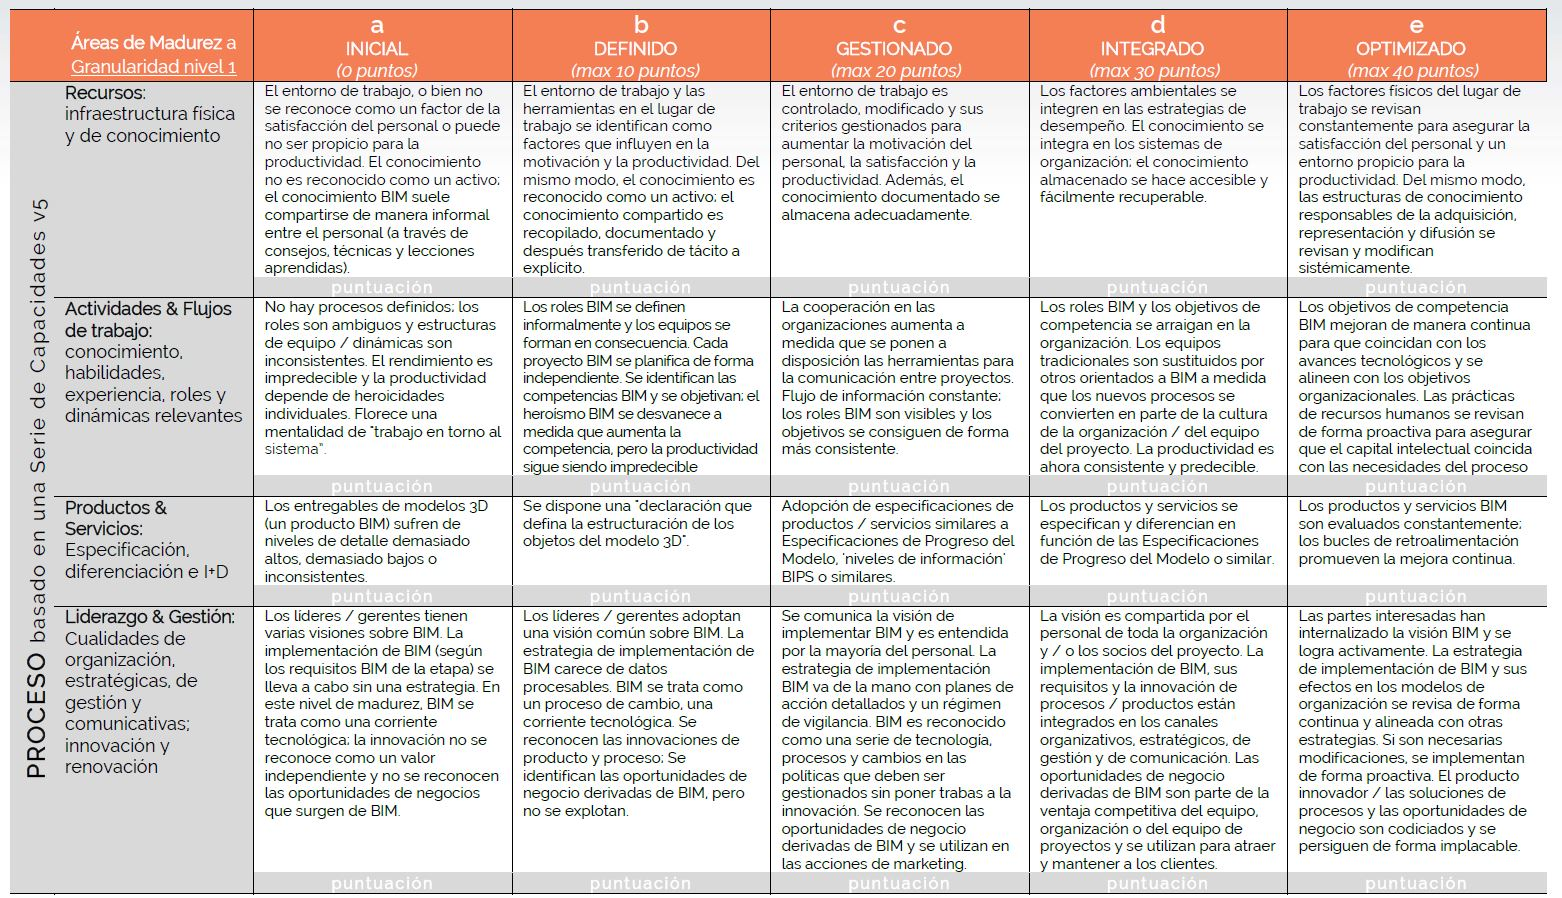
\includegraphics[width=1\linewidth]{images/matriz-madurez-2.jpeg}
    \caption{Matriz basada en el proceso.}
\end{figure}

\begin{figure}[H]
    \centering
    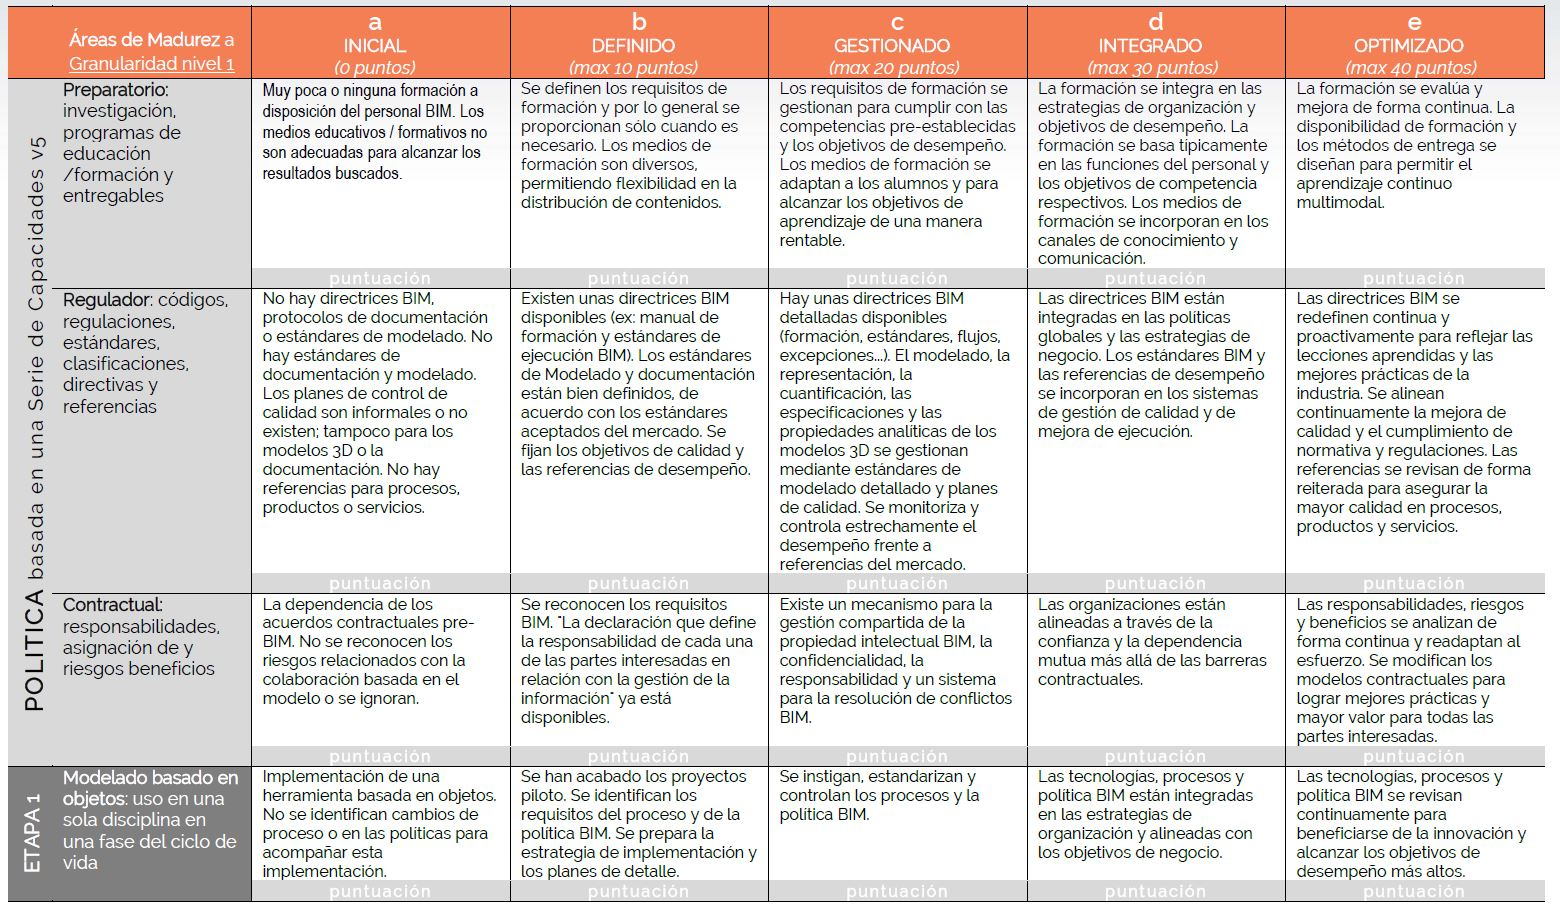
\includegraphics[width=1\linewidth]{images/matriz-madurez-3.jpeg}
    \caption{Matriz basada en la política.}
\end{figure}

\section{Códigos de los desarrollos}

\subsection{Herramienta de transformación de la data}

\begin{lstlisting}[language=Python]
import pandas as pd
import numpy as np
import os, glob

data = input('Nombre archivo:')
monto = float(input('Monta base:'))
variacion = float(input('Variacion:'))

def contracts(data, monto, variacion):
    path = (os.getcwd() + '/data/' + data).replace('\\','/')
    df = pd.read_excel(path, header=7)
    df.drop(df.columns[[1,2,4,5,6,7,8]], axis=1, inplace=True)
    df.columns = ['Contrato', 'Descripcion', 'Total']
    df.dropna(subset=['Total'], how='any', inplace=True)

    contrato = (df[df['Contrato'].str.contains('nombre', case=False)]
                                 .iloc[:,0])
                                 .reset_index(drop=True)
    base = (df[df['Contrato'].str.contains('revision 0.0', case=False)]
                             .iloc[:,2])
                             .reset_index(drop=True)
    cierre = (df[df['Contrato'].str.contains('total compro', case=False)]
                               .iloc[:,2])
                               .reset_index(drop=True)

    df1 = pd.concat([contrato, base, cierre], axis=1)
    df1.columns = ['Contrato', 'Base', 'Cierre']
    df1['Delta'] = df1['Cierre'] - df1['Base']

    #Remueve los primeros 8 caracteres del string en la columna 'Contratos'
    df1['Contrato'] = df1.Contrato.str.slice(start=8) 
    df1['Variacion'] = df1['Delta']/(df1['Base'] + 0.00000001)

    df2 = df1[df1.Delta > 0].reset_index(drop=True)
    
    df3 = (df2[(df2['Base'] > monto) & (df2['Variacion'] > variacion)])
                .sort_values(by=['Base'], ascending=False)
                .reset_index(drop=True)

    return df, df1, df2, df3

df, df1, df2, df3 = contracts(data, monto, variacion)

def contract_analysis_base(df, monto, variacion):

    dfs = df[df.Contrato.str.match('0.0|nombre|revision 0.0|total compro', 
                                   case=False)]
                                   .reset_index(drop=True)
    dfs[dfs['Descripcion'].str.contains('suministr', 
                                         case=False)==True]

    ind_nombre = dfs[dfs['Contrato'].str.contains('nombre', 
                                                   case=False)]
                                    .index
                                    .tolist()
    ind_base = dfs[dfs['Contrato'].str.contains('revision 0.0', 
                                                 case=False)]
                                  .index
                                  .tolist()
    ind_cierre = dfs[dfs['Contrato'].str.contains('total compro', 
                                                  case=False)]
                                    .index
                                    .tolist()
    ind_df = pd.DataFrame(np.column_stack([ind_nombre, 
                                        ind_base, 
                                        ind_cierre]), 
                                        columns=['indice contrato', 
                                                 'indice base', 
                                                 'indice cierre'])

    l = []
    for i in range(len(ind_df)):
        if (dfs.Total[ind_df['indice base'][i]] > monto) 
            and 
           (dfs.Total[ind_df['indice cierre'][i]] /
           dfs.Total[ind_df['indice base'][i]] - 1 > variacion):

            s = dfs.iloc[ind_df['indice contrato'][i]
                    :ind_df['indice base'][i], :]
            l.append(s)
            dfx = pd.concat(l, ignore_index=True) 
        
    return dfx

df_base = contract_analysis_base(df, monto, variacion)

def contract_selection(df, monto, variacion):

    df4 = (df[~df['Contrato']
            .str.match('0.0|totales fina', case=False)])
            .reset_index(drop=True) 

    ind_nombre = df4[df4['Contrato']
                .str.contains('nombre', case=False)]
                .index.tolist()
    ind_base = df4[df4['Contrato']
                .str.contains('revision 0.0', case=False)]
                .index.tolist()
    ind_cierre = df4[df4['Contrato']
                .str.contains('total comprom', case=False)]
                .index.tolist()
    ind_df = pd.DataFrame(np.column_stack([ind_nombre, 
                                          ind_base, 
                                          ind_cierre]), 
                            columns=['indice contrato', 
                                     'indice base', 
                                     'indice cierre'])

    l = []
    for i in range(len(ind_df)):
        if (df4.Total[ind_df['indice base'][i]] > monto)
            and (df4.Total[ind_df['indice cierre'][i]]/
                df4.Total[ind_df['indice base'][i]] - 1 > variacion):
            s = df4.iloc[ind_df['indice contrato'][i]
                    :ind_df['indice cierre'][i]+1, :]
            l.append(s)
            df5 = pd.concat(l, ignore_index=True) 

    df5['Contrato'] = df5.Contrato
                         .str.replace('Revision 0.0 - Totales', 
                                      'Costo Base',
                                       regex=False)
    df5['Contrato'] = df5.Contrato
                         .str.replace('Total Compromiso', 
                                      'Costo Final', 
                                       regex=False)
    df5 = df5[~df5.Contrato
                  .str.contains('revision', case=False)]
    return df5

df_s = contract_selection(df, monto, variacion)

resumen = df_s[df_s.Contrato
                   .str.contains('nombre|costo base|costo final', 
                                case=False)]
del resumen['Descripcion']

with pd.ExcelWriter('selected_contracts_(from code).xlsx') as writer:
    df1.to_excel(writer, 
                sheet_name='Reagrupacion', 
                index=False)
    df2.to_excel(writer, 
                 sheet_name='Solo crecimientos', 
                index=False)
    df3.to_excel(writer, 
                 sheet_name='Seleccionados', 
                 index=False)
    df_s.to_excel(writer, 
                  sheet_name='Detalle seleccionados', 
                  index=False)
    resumen.to_excel(writer, 
                     sheet_name='Resumen seleccionados', 
                     index=False)

items = ['extension plazo', 
         'obras adicionales', 
         'materiales', 
         'ingenieria']

key_words = ['extension plazo|plazo', 
            'montaje|obras adicio|adicional
            |extraordinaria|obraexcav|civil|rellen
            |reempla|reparaci|instalaci', 
            'hormig|piping|caner|tuber|valvula
            |valv|pern|sumin|adqui|estruc|acero', 
            'ingenieri|cambios alcan|ingenieria de terreno
            |ingenieria de terreno'] 

def cost_deviations(df, key_words):
    l = []
    for i in range(len(key_words)):
        a = df[df['Descripcion'].str
                                .contains(key_words[i], 
                                          case=False)==True] 
        l.append(a)
        df = df.merge(l[i].drop_duplicates(), 
                            on=['Contrato', 
                                 'Descripcion', 
                                 'Total'], 
                                 how='left', 
                                 indicator=True)
        df = df[df['_merge'] =='left_only']
        del df['_merge']

    return l

l = cost_deviations(df_s, key_words)

def resumen_items(l, items):
    d = {}
    a = 0 
    for i in range(len(items)):       
            d[items[i]] = l[i].Total.sum()
            a += l[i].Total.sum()
            
    d['Total'] = a
    dff = pd.DataFrame(d, index=['USD', 'Var']).T
    dff.Var = dff.USD/df2.Base.sum()

    return dff

dff = resumen_items(l, items)

dx = resumen_items(cost_deviations(df_base, key_words), items)

with pd.ExcelWriter('cost_deviations_(from code).xlsx') as writer:
    dff.to_excel(writer, 
                 sheet_name='Resumen seleccionados', 
                 index=True)
    dx.to_excel(writer, 
                sheet_name='Resumen seleccionados base', 
                index=True)
    for i in range(len(items)):
        pd.DataFrame(l[i]).to_excel(writer, 
                                    sheet_name=items[i], 
                                    index=False)
\end{lstlisting}

\subsection{Herramienta de estimación de los parámetros}

\begin{lstlisting}[language=Python]
import pandas as pd
import statsmodels.api as sm
import os

def main():
    path:str = os.getcwd() + "/data.csv"

    # Matriz de datos globales
    data_df = pd.read_csv(path)
    data_df["indicador_madurez"] = 4 / data_df["madurez_succar"]
    data_df["const"] = 1

    # Matrices Y y X
    y_data = data_df["desv_costos"]
    x_data = data_df[["const", "indicador_madurez"]]

    regression = sm.OLS(endog=y_data, 
                        exog=x_data,
                        missing="drop")
    result_reg = regression.fit()
    result_summary = result_reg.summary()

    print(result_summary)
    print("\nDATA INGRESADA PARA LA ESTIMACION\n")
    print(data_df)

    
if __name__ == "__main__":
    main()
\end{lstlisting}


\end{document}